\documentclass[UTF8]{beamer}
\usepackage{graphicx, color}
\usepackage{algorithm2e}
\usepackage{zhspacing}
\usepackage{amsmath}

\usepackage{underscore}
\usetheme{JuanLesPins}
\usepackage{fontspec}
\setsansfont{Microsoft YaHei}

\usepackage{enumerate}

\AtBeginSection[]{
  \frame{
    \frametitle{Next}
    \tableofcontents[currentsection, subsectionstyle=show/shaded/hide]
  }
}

\title{Programming in Real Bioinformatics}

\author{Gang Chen\\ chengang@bgitechsolutions.com}

\logo{
\includegraphics[width=1.3cm]{bgi-logo.png}
\includegraphics[width=2.5cm]{cuhklogo.png}}
\date{\today}




\begin{document}

\begin{frame}
\titlepage
\end{frame}

\begin{frame}[t]\frametitle{Outline}
\tableofcontents[hideallsubsections]
\end{frame}

\section{Five Programming Languages?}
\begin{frame}
  \frametitle{Why do we need five programming languages?}
  \begin{block}{Why do we have to learn languages?}
  \begin{itemize}
    \item 廣東話
    \item 普通话
    \item 客家话
    \item 上海话
    \item English
    \begin{itemize}
      \item England, Scotland, Wales, North Ireland
      \item United States
      \item Hong Kong
    \end{itemize}
    \item Hinglish
    \item \ldots
  \end{itemize}
\end{block}
\end{frame}

\begin{frame}
  \frametitle{Programming Languages}
  \tiny
  \begin{itemize}
    \item C: Embedded device, high performance system software
    \item C++: Embedded device, large-scale software, GUI applications
    \item Java: Large-scale system, Enterprise systems, cross-platform applications
    \item Perl: Text processing, biological sequence processing, CGI-programming
    \item Python: System administration, desktop applicatons, web development
    \item R: Data analysis and visualization
    \item Objective-C: applications on iOS and Mac OS
    \item Swift: a future programming languages for Apple products
    \item Go: Google's system programming languages
    \item Ruby, Scala, Julia, JavaScript, LaTeX \ldots
  \end{itemize}
\end{frame}

\begin{frame}
  \centerline{
\includegraphics[height=\textheight]{slsw.jpg}}
\end{frame}

\begin{frame}
  \centerline{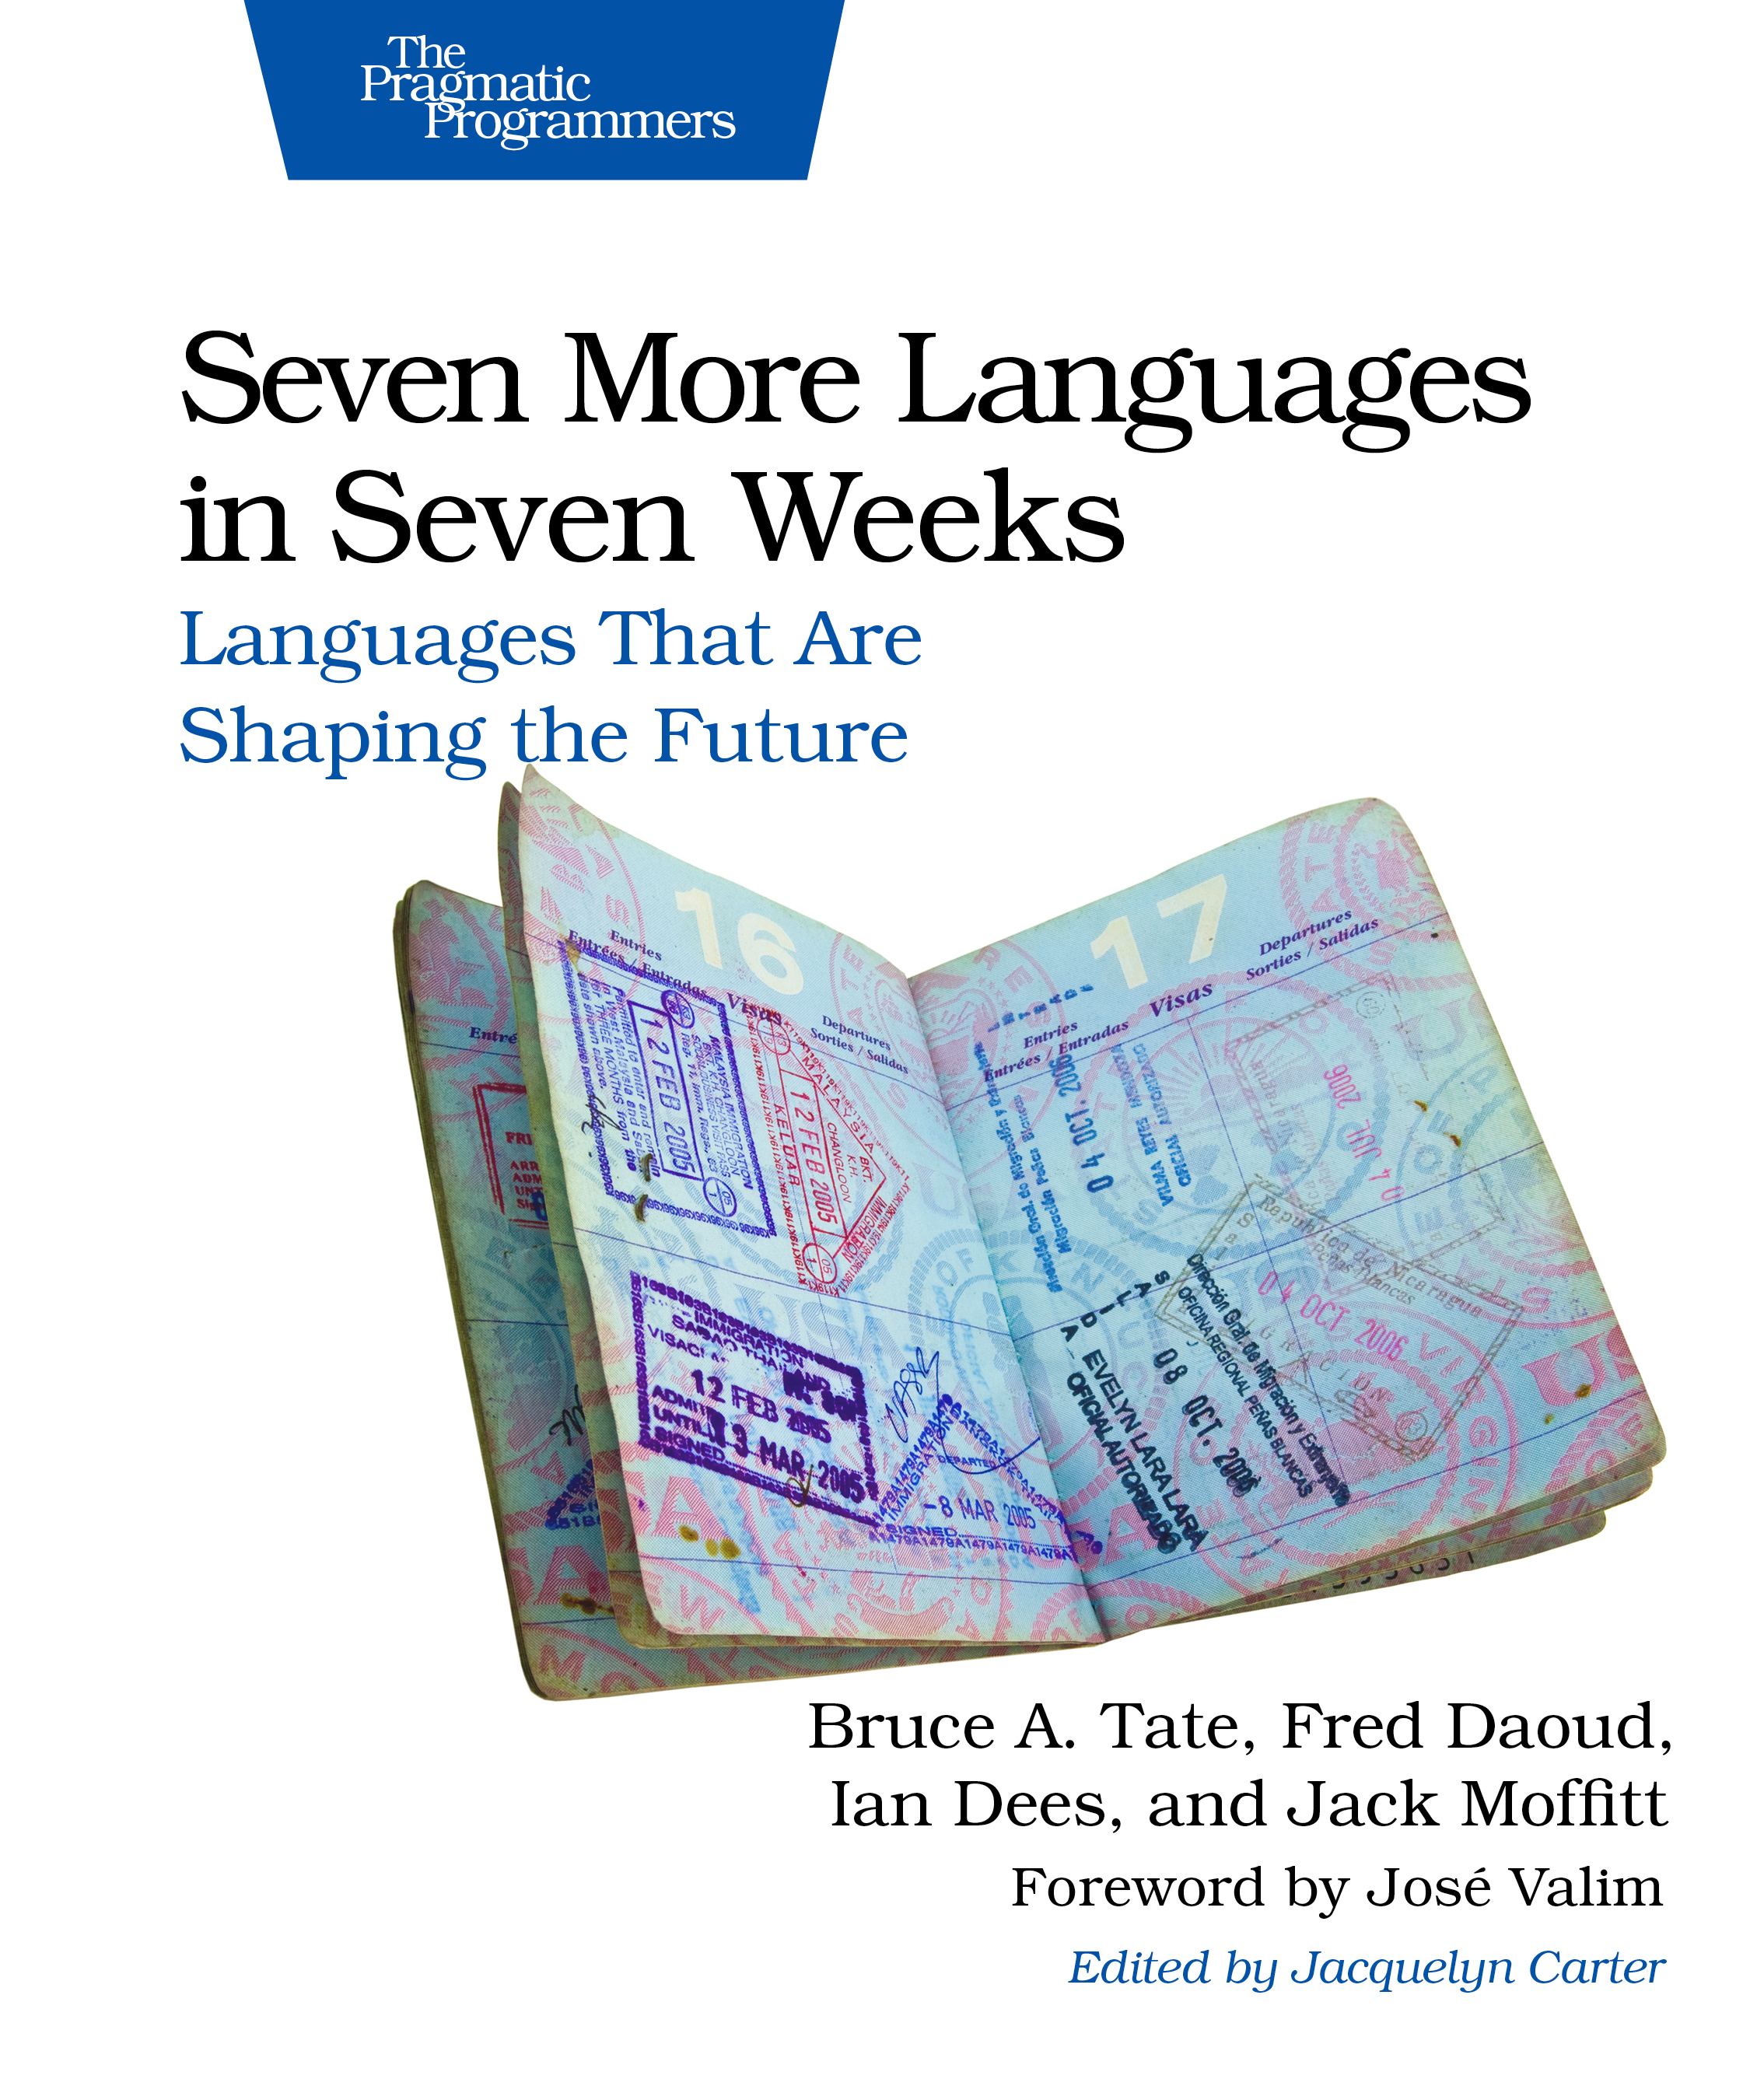
\includegraphics[height=\textheight]{smlsw.jpg}}
\end{frame}

\begin{frame}
  \centerline{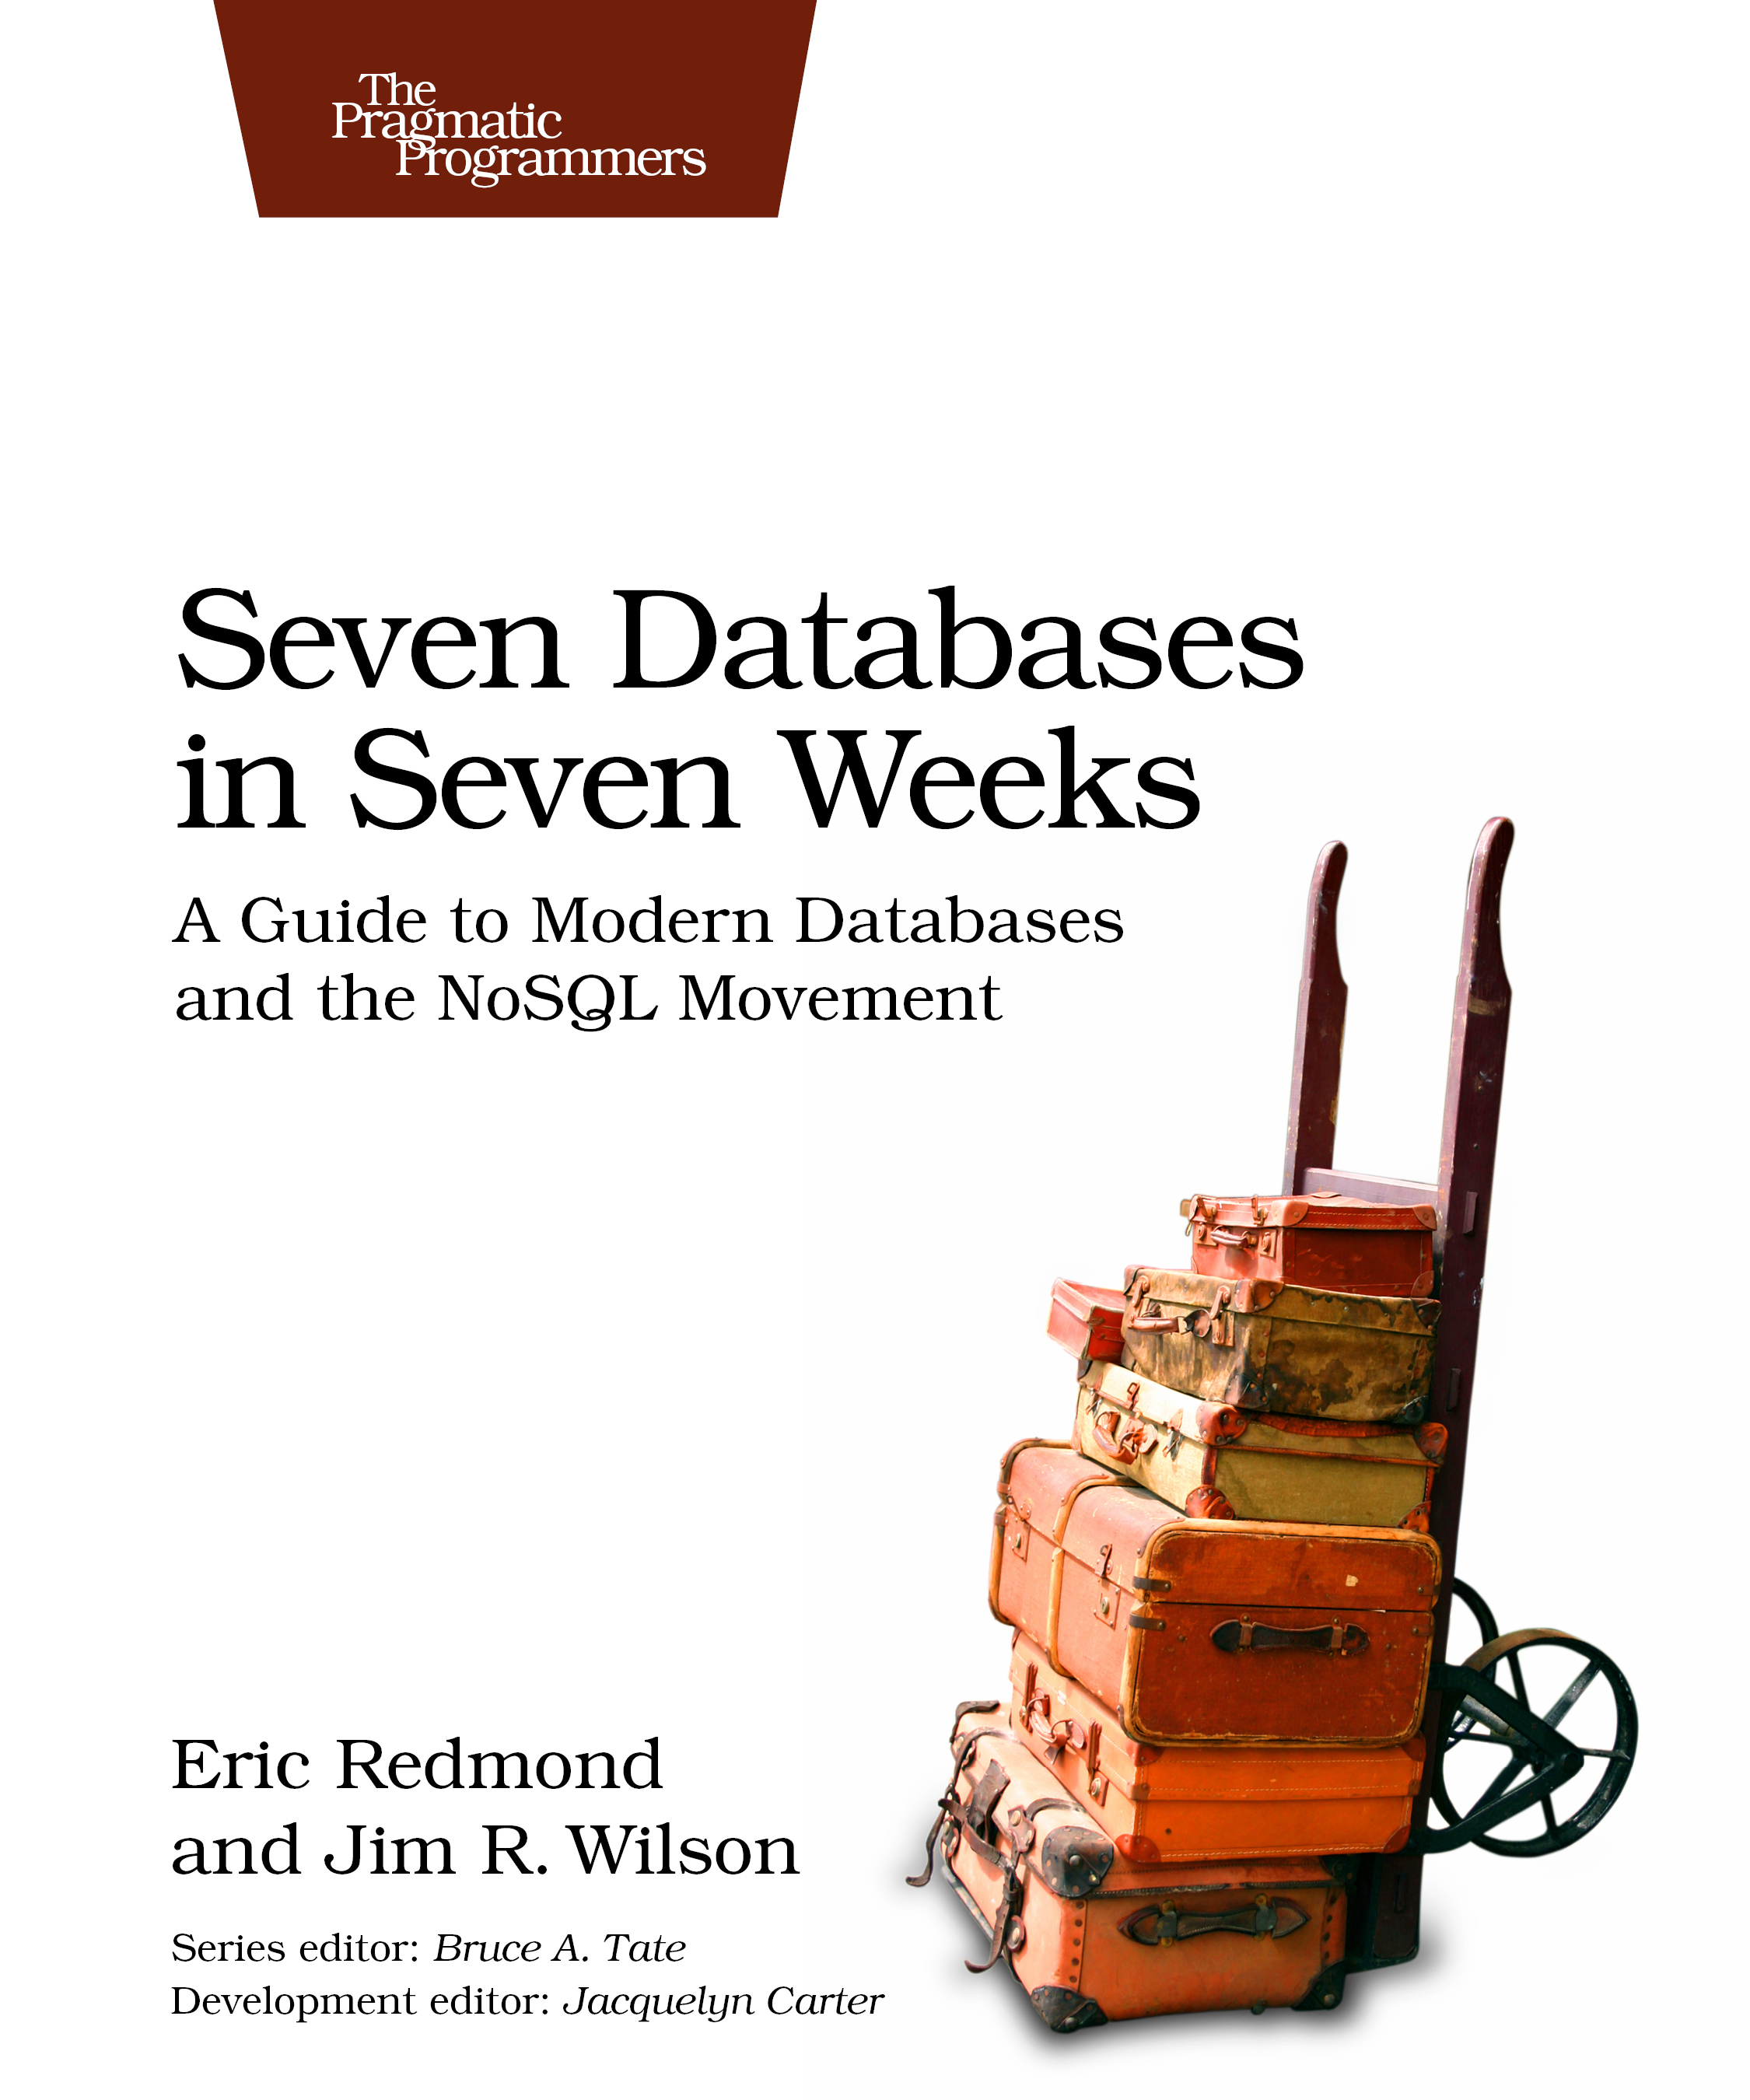
\includegraphics[width=.33\textwidth]{sdsw.jpg}
  
\includegraphics[width=.33\textwidth]{scmsw.jpg}
  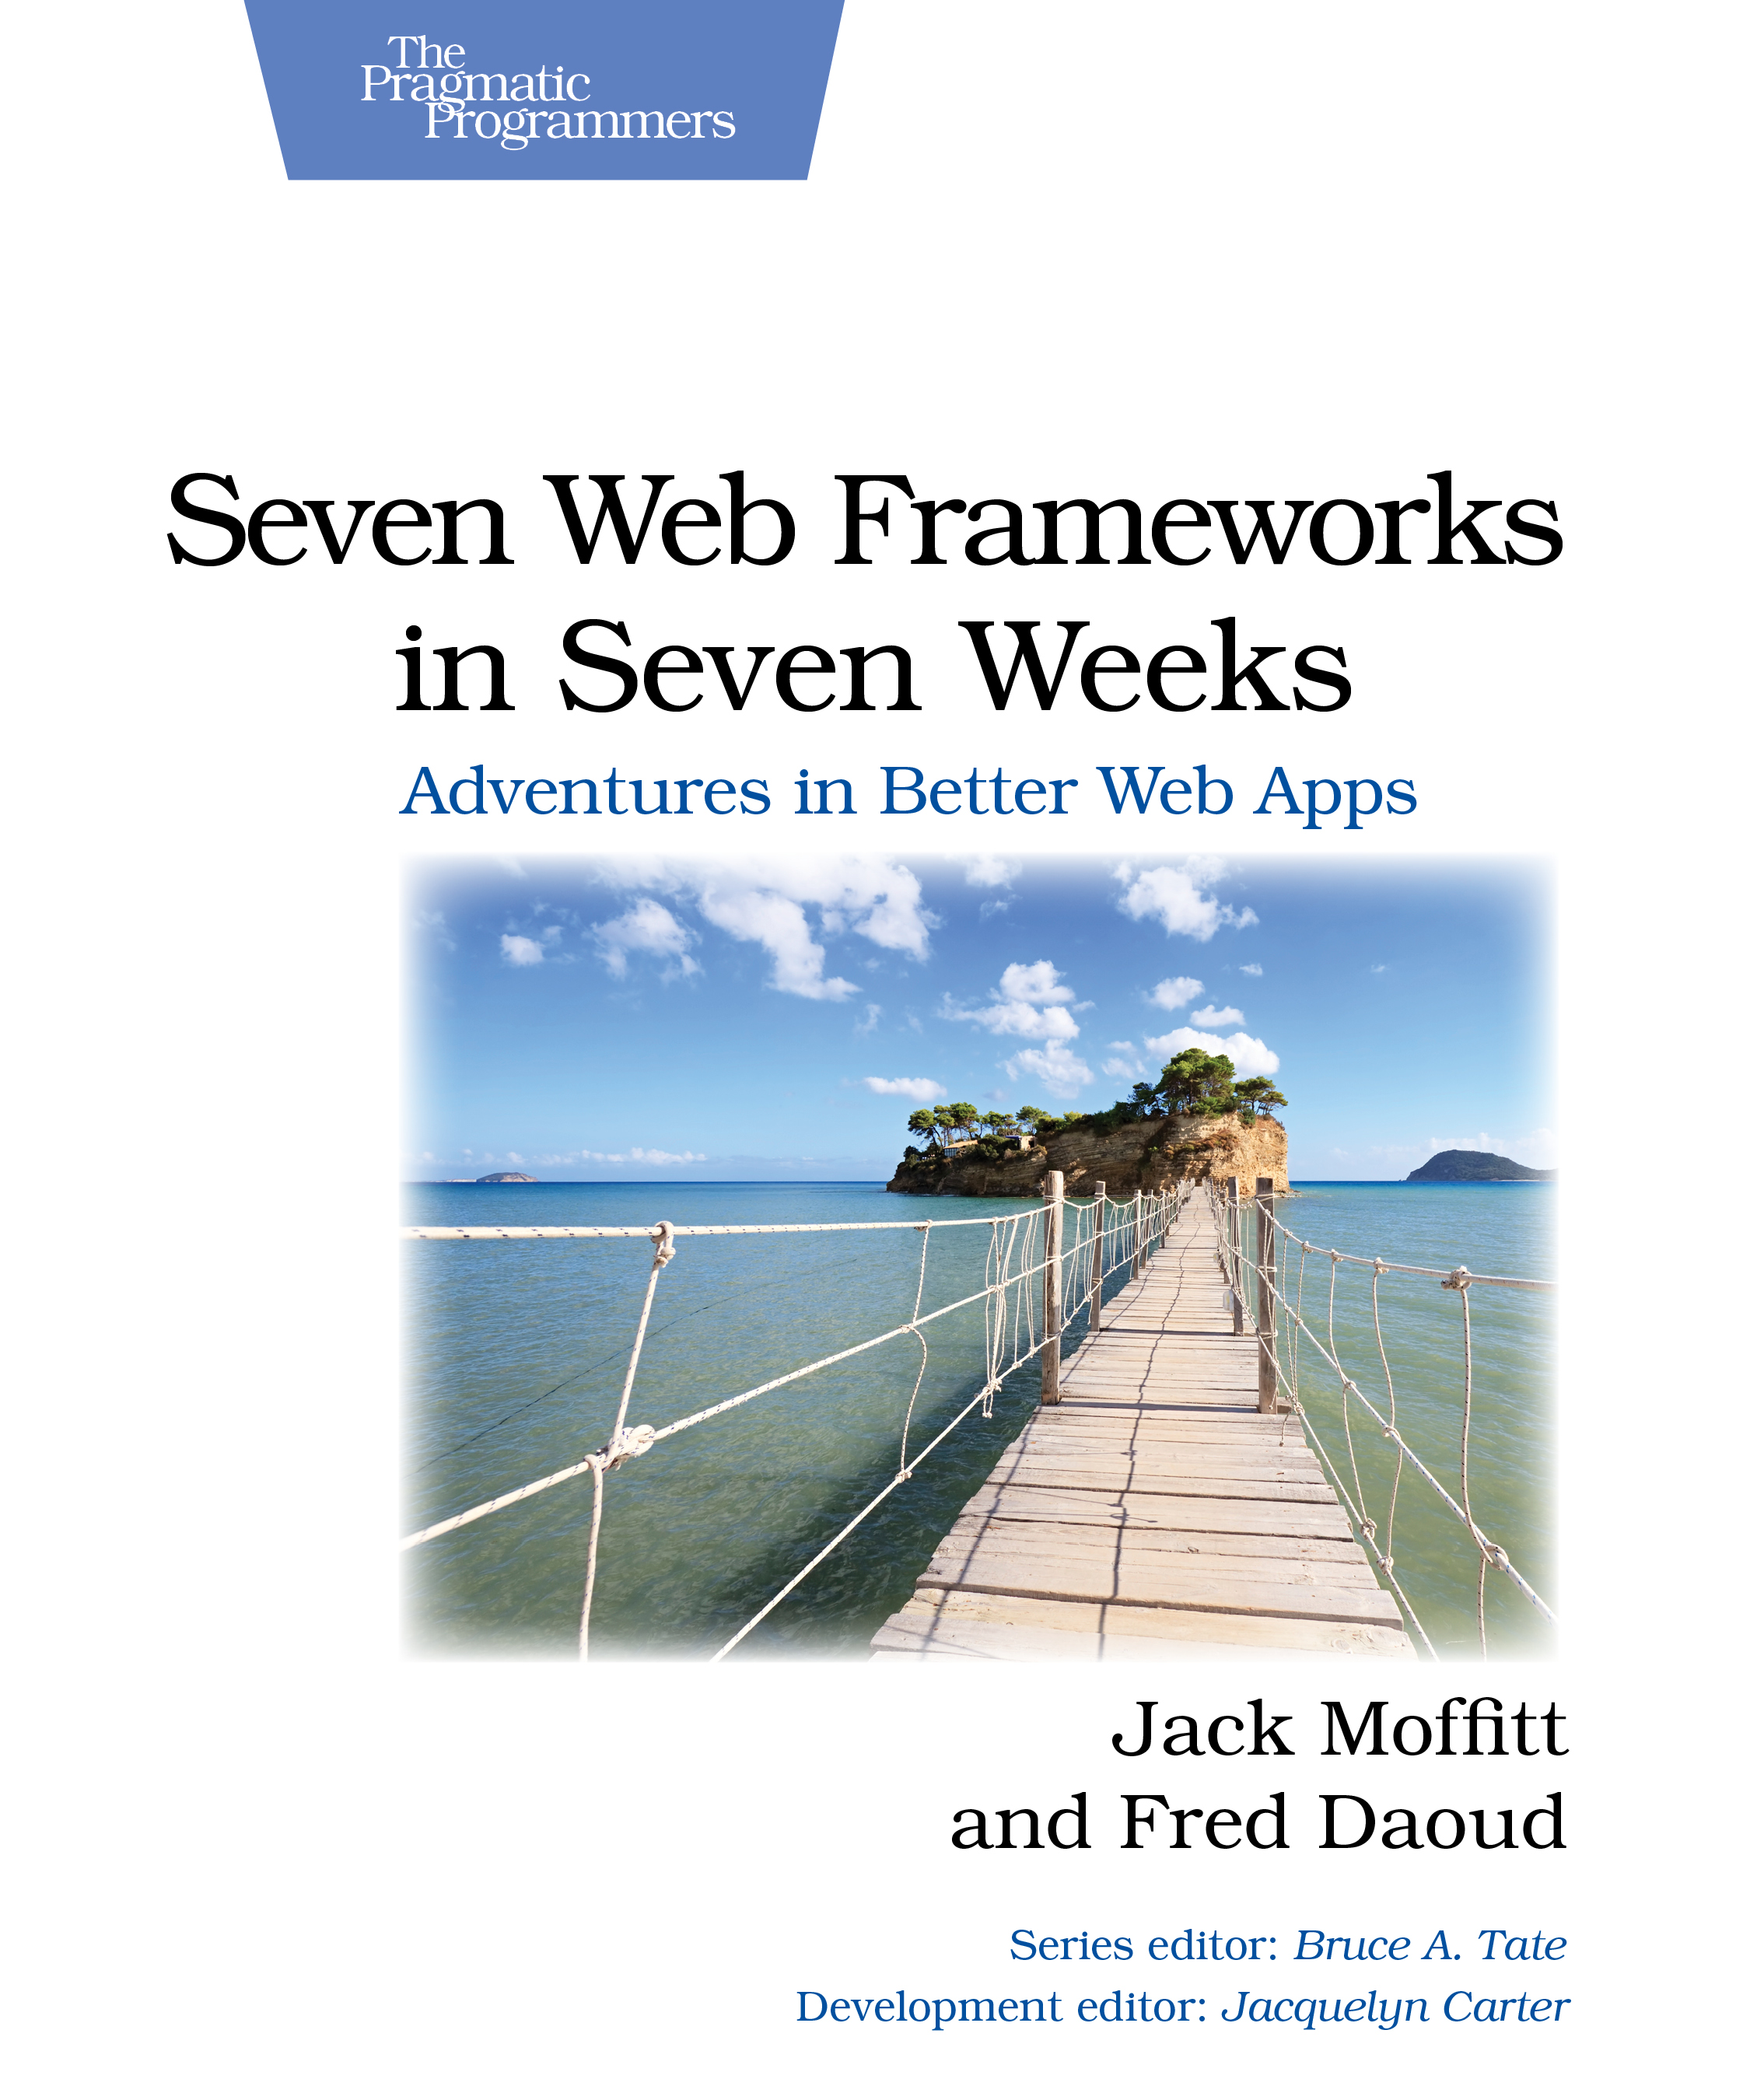
\includegraphics[width=.33\textwidth]{swfsw.jpg}}
\end{frame}

\begin{frame}
  \frametitle{Interaction between Programming Languages}
  \begin{itemize}
    \item C-based: C, C++, Go, R, Perl, Python \ldots
    \item Virtual Machine based:
    \begin{itemize}
      \item JVM: Java, Scalar, JPython, Perl 6 \ldots
      \item CLI: C++/CLI, C\#, IronPython, F\#, VB.NET, PowerShell \ldots
    \end{itemize}
    \item Interface: web service, file, database, container \ldots
  \end{itemize}
\end{frame}

\begin{frame}
  \begin{itemize}
    \item Java and R: rJava
    \item Perl and R: RSPerl
    \item Python and R: rpy2
    \item C/C++ and R: Rcpp
    \item C and Perl: perl.h
    \item Java and C/C++: JNI
  \end{itemize}
\end{frame}


\section{Software Development Process}

\section{Waterflow}
\begin{frame}
  \frametitle{Waterflow}
  \centerline{\includegraphics[height=.8\textheight]{waterflow.png}}
\end{frame}

\begin{frame}
  \frametitle{Case: Fibonacci Sequence Generator}
\end{frame}

\section{Agile Software Development}

\begin{frame}
  \frametitle{Case: Fibonacci Sequence Generator}
\end{frame}

\section{Conclusion}

\section{Final Examination}
\begin{frame}
  \frametitle{Scope}
\end{frame}

\begin{frame}
  \frametitle{Question Sample}
\end{frame}

\begin{frame}
  \frametitle{Question Sample}
\end{frame}

\begin{frame}
  \frametitle{Tips}
\end{frame}

\end{document}
